    \begin{lstlisting}[language=alloy]
module CodeKataBattle


//These can be Enum
abstract sig Language {}
one sig PYTHON extends Language {}  
one sig JAVA extends Language {}
one sig C extends Language {}
one sig CPP extends Language {}
one sig JAVASCRIPT extends Language {}
one sig RUBY extends Language {}
one sig GO extends Language {}
one sig RUST extends Language {}
one sig CSHARP extends Language {}
abstract sig QualityAspect {}
one sig COMPLEXITY, DUPLICATIONS, MAINTAINABILITY, RELIABILITY, SECURITY, CLEAN_CODE extends QualityAspect {}

//These can be Enum
abstract sig  TournamentStatus {}
one sig REG_OPEN, ONGOING, CLOSED extends TournamentStatus{}
//These can be Enum
abstract sig BattleStatus {}
one sig REG_OPEN_BATTLE, ONGOING_BATTLE, CONSOLIDATION, CLOSED_BATTLE extends BattleStatus{}

// Basic types
abstract sig Bool {}
one sig TRUE extends Bool {} 
one sig FALSE extends Bool {}

sig Time{
time: one Int
} {time>0}

//These fields are removed from User for the sake of simplicity because they are not related to anything but user specific attributes.  They can be unique or same, no check in the system related to this.
//sig Password{}
//sig Name{}
//sig Surname{}

abstract sig Notification{}
sig TournamentCreated extends Notification{
  tournamentCreated: one Tournament
}
sig TournamentEnded extends Notification{
tournamentEnded: one Tournament
}
sig TournamentInvited extends Notification{
tournamentInvited: one Tournament
}
sig BattleStarted extends Notification{
battleStarted: one Battle
}
sig BattleFinished extends Notification{
battleFinished: one Battle
}

sig Institution{}
sig TournamentTitle{}
sig TournamentDescription{}

sig TeamName{}

sig URL{}

sig Email{}
sig User {
    email: one Email,
    notifications: set Notification
}

sig Educator extends User {
    var creates: set Tournament,
    var contributesTo: set Tournament,
    var createsBattle: set Battle,
    institutions: set Institution,
    var givenManualScores: set ManualScore
}

sig Student extends User {
    var registers: set Tournament,
    var tournamentScores: Tournament -> lone Int,
    institution: lone Institution,
}

sig Tournament {
    title: one TournamentTitle,
    description: one TournamentDescription,
    registrationDeadline: one Time,
    closingTime: lone Time,
    var status: one TournamentStatus,
    var hasBattle: set Battle,
    var subscribers: set Student,
} {
     registrationDeadline.time < closingTime.time

}

sig ScoringWeights{
    TEST_CASES:  Int,
    TIMELINESS:  Int,
    QUALITY:  Int
    } {
     TEST_CASES > 0 && TIMELINESS > 0 && QUALITY>0 && plus[plus[TEST_CASES,TIMELINESS],QUALITY]=6
    }
	
sig Team {
    teamName: one TeamName,
    hasMember: some Student,
    submits: lone Submission,
}

sig BattleTitle {}
sig Battle {
    title: one BattleTitle,
    codeKata: one CodeKata,
    minStudentsPerGroup: one Int,
    maxStudentsPerGroup: one Int,
    creationTime: one Time,
    registrationDeadline: one Time,
    submissionDeadline: one Time,
    var status: BattleStatus,
    allowedLanguages: some Language,
    chosenQualityAspects: some QualityAspect,
    var teams: set Team,
    scoringWeights: one ScoringWeights,
    manualScoringEnabled: one Bool,
    battleRepositoryUrl: lone URL,
    sandboxEnvironment: SandboxEnvironment,
} {
  registrationDeadline.time < submissionDeadline.time &&
  minStudentsPerGroup<=maxStudentsPerGroup &&
  minStudentsPerGroup>=0 &&
  maxStudentsPerGroup>=0 
 }

sig Code{}
sig Submission{
code: one Code,
repositoryUrl: one URL,
commitTime: one Time,
score: one BattleScore,
sandboxEnvironment: SandboxEnvironment
}
sig ManualScore{
    score: one Int
} {score>=0}
sig BattleScore {
    testCasesScore: one Int,
    timelinessScore: one Int,
    qualityScore: one Int,
    manualScore: lone ManualScore,
    totalScore: one Int
} {
   totalScore = calculateBattleScore[this]
   testCasesScore >=0
   timelinessScore >=0
   qualityScore >= 0
}

fun calculateBattleScore(bs:BattleScore): Int {
    bs.testCasesScore + bs.timelinessScore + bs.qualityScore
}

sig BattleDescription{}
sig CodeKata {
    description: one BattleDescription,
    testCases: some TestCase,
    buildScripts: some BuildScript
} 

sig TestCase {
language: one Language
}

sig BuildScript {
language: one Language
}


//Each  battle has a sandbox environment that runs the code
sig SandboxEnvironment{}

// Relationships and constraints


//Every user has unique email 
fact EmailsAreUnique{
no disjoint u1, u2: User | u1.email = u2.email
}

//Every user is eiher Educator or Student
fact AllUsersAreEitherEducatorOrStudent {
    all u: User |
        (u in Educator and u not in Student) or (u in Student and u not in Educator)
}

// Each team must be associated with a battle and have members within the specified group size constraints.
fact TeamsWithinGroupSizeConstraints {
    all t: Team |some b: Battle	|	t in b.teams	and	#t.hasMember >= b.minStudentsPerGroup and #t.hasMember <= b.maxStudentsPerGroup
}

//In a battle there must be test cases and build scripts for each allowed language
fact ArtifactsProvided {
    all b: Battle | {
        all l: b.allowedLanguages | {
            one tc: TestCase | tc.language=l	and	tc in b.codeKata.testCases
            one bs: BuildScript| bs.language=l and bs in b.codeKata.buildScripts
        } 
    }
}

//no other than allowed languages
fact TestCasesAndBuildScriptsForAllowedLanguagesOnly {
    all b: Battle | 
            b.codeKata.testCases.language in b.allowedLanguages and b.codeKata.buildScripts.language in b.allowedLanguages
}



// Each Test Case and Build Script Belongs To One Code Kata
fact ArtifactsBelongsToOneCodeKata {
    // For every TestCase, there is exactly one CodeKata that it's related to
    all tc: TestCase | one ck: CodeKata | tc in ck.testCases
    
    // For every BuildScript, there is exactly one CodeKata that it's related to
    all bs: BuildScript | one ck: CodeKata | bs in ck.buildScripts
}

// Every tournament is created by exactly one educator
fact UniqueEducatorForTournament {
    all t: Tournament | one e: Educator | e.creates = t
}

fact UniqueBattleForCodeKata {
    // Every CodeKata is associated with exactly one Battle
    all ck: CodeKata | one b: Battle | ck = b.codeKata
}


// Every tournament is contributed to by at least one educator which is the creator of the tournament
fact CreatorContributesTournament {
    all t: Tournament | one e: Educator | t = e.creates and t in e.contributesTo
}

// Every battle is created by exactly one educator
fact UniqueCreatorForBattle {
    all b: Battle | one e: Educator | e.createsBattle = b
}

// Every battle is associated with exactly one tournament
fact UniqueTournamentForBattle {
    all b: Battle | one t: Tournament | b in t.hasBattle and 
        all tOther: Tournament - t | b not in tOther.hasBattle
}

//for consitency
fact SubscribersAreRegistered {
    all t: Tournament, s: Student |  t in s.registers implies s in t.subscribers 
}



// Every educator can create battles only for tournaments they contribute to
fact ContributerCreatesBattle{
    all e: Educator, b: Battle | b in e.createsBattle implies b in e.contributesTo.hasBattle
}

// Unique battle titles within a tournament
fact UniqueBattleTitle{
    all t: Tournament | no disjoint b1, b2: t.hasBattle | b1.title = b2.title
}

// Unique tournament titles
fact UniqueTournamentTitles {
    no disjoint t1, t2: Tournament | t1.title = t2.title
}

// Unique team names within a battle
fact UniqueTeamNamesWithinBattle {
    all b: Battle | no disjoint t1, t2: b.teams | t1.teamName = t2.teamName
   all tn:TeamName	|	one t: Team	|	t.teamName=tn
}

// Ensure submission constraints
fact EveryManualScoreHasAScoreAndSubmission {
    all ms: ManualScore | 
        one bs: BattleScore | bs.manualScore = ms
}

fact EveryManualScoreHasAScoreAndSubmission {
    all bs: BattleScore | 
        one s: Submission | bs in s.score
}

fact EveryManualScoreHasAScoreAndSubmission {
    all s: Submission | 
        one t: Team | s in t.submits
}

fact EveryManualScoreHasAScoreAndSubmission {
    all t: Team | 
        one b: Battle | t in b.teams
}


fact EveryCodeHasASubmission {
    // For every Code, there exists a Submission that has this score
    all cd: Code | one s: Submission | s.code = cd
}

// A student's submission must be their own work and associated with a team that is part of a battle. A domain assumption
fact UniqueSubmissionRepositoryUrlWithinBattle {
    all url: URL | one s: Submission | s.repositoryUrl = url
}

// A student can only be part of at most one team per battle
fact StudentInAtMostOneTeamPerBattle {
    all b: Battle | no disj t1, t2: b.teams | some s: Student | s in t1.hasMember and s in t2.hasMember
}


// Students can only be part of teams for battles in tournaments they have registered for.
fact StudentTeamRegistrations {
    all s: Student | all t: s.registers | let battles = t.hasBattle |
    all team: Team | s in team.hasMember implies team in battles.teams
}


// There is no created battle if tournament status is REG_OPEN
fact noBattlesInRegistration {
    all t: Tournament | t.status = REG_OPEN implies no t.hasBattle
}

// There is no submission  if battle status is REG_OPEN_BATTLE
fact noSubmissionsAndRepoForOpenBattles {
    all b: Battle | b.status = REG_OPEN_BATTLE implies {
        no t: b.teams | some t.submits and
        no b.battleRepositoryUrl
    }
}


fact AllBattlesClosedIfTournamentClosed {
    all t: Tournament | t.status = CLOSED implies all b: t.hasBattle | b.status = CLOSED_BATTLE
}


// Battle registration time is less than Tournament closing Time. It is check for closed tournaments. A closed tournament can not have a battle with creation time later than closing time
fact BattlesWithinTournamentClosingTime {
    all t: Tournament, b: t.hasBattle | one t.closingTime && b.creationTime.time < t.closingTime.time
}

fact ManualScoreConstraint {
    all bs: BattleScore |
       one  bs.manualScore  implies bs.manualScore.score >= 0 && bs.manualScore.score <= 2
}


//Scores should be in range 0 and their weights
fact ScoreWithinWeightRange {
    all t: Team | some t.submits implies {
        let s = t.submits.score |
            // Find the battle that includes this team
            some b: Battle | t in b.teams and {
                let weights = b.scoringWeights |
                s.testCasesScore >= 0 and s.testCasesScore <= weights.TEST_CASES and
                s.timelinessScore >= 0 and s.timelinessScore <= weights.TIMELINESS and
                s.qualityScore >= 0 and s.qualityScore <= weights.QUALITY
            }
    }
}

fact enforceManualScoringRules {
    all b: Battle | {
        // If the battle is in consolidation and manual scoring is enabled,
        // there must be a manual score for each battle score
        (b.status = CLOSED_BATTLE and b.manualScoringEnabled = TRUE) implies {
            all s: b.teams.submits.score | some ms: ManualScore | ms in s.manualScore
        }
        
        // If manual scoring is not enabled, the status cannot be CONSOLIDATION
        (b.manualScoringEnabled = FALSE) implies b.status != CONSOLIDATION
        
        // If the battle is in before consolidation or manual scoring is not enabled,
        // there cannot be a manual score for any battle score
        (b.status = REG_OPEN_BATTLE  or b.status = ONGOING_BATTLE or b.manualScoringEnabled = FALSE) implies {
            all s: b.teams.submits.score | no s.manualScore
        }
    }
}


//This fact enforces the rule that if a ManualScore exists for a BattleScore in a Battle, 
//it must have been given by the Educator who created that Battle. 
//If there is no ManualScore, this fact does not impose any additional requirements.
// In other words, it only applies when a ManualScore is present.
fact manualScoresGivenByCreator {
    all b: Battle, s: b.teams.submits.score, ms: s.manualScore | {
        some e: Educator | e.createsBattle = b and ms in e.givenManualScores
    }
}

//if a tournament is created (exists), it should be in Student's notification with as TournamentCreated notification, for every tournament exist there must be a notification about it in their notifications field.
fact notificationForTournamentCreation {
    all t: Tournament, s: Student | 
        one n: s.notifications | n in TournamentCreated and n.tournamentCreated = t
}

//if tournament is ended (status is CLOSED), it should be in Student's notification with as TournamentEnded notification, for every tournament ended there must be a notification about it in their notifications field.
fact notificationForTournamentEnding {
    all t: Tournament | t.status = CLOSED implies 
        all s: Student | s in t.subscribers implies 
            one n: s.notifications | n in TournamentEnded and n.tournamentEnded = t
}

fact TournamentEndedNotificationMeansTournamentEnded {
    all n: TournamentEnded | n.tournamentEnded.status = CLOSED
}


// if an educator is contributes to a tournament but not a creator, there must be a notification in its notifications with a TournamentInvited notification. 
fact notificationForEducatorInvitation {
    all e: Educator, t: Tournament | t in e.contributesTo  and t not in  e.creates implies
        one n: e.notifications | n in TournamentInvited and n.tournamentInvited = t
}

//if a battle is not in REG_OPEN_STAGE, there must be a BattleStarted Notification of the  notification field of students enrolled in that battle. For every battle started there must be one .
fact notificationForBattleStarting {
    all b: Battle, s:Student |	 b.status != REG_OPEN_BATTLE and s in b.teams.hasMember implies 
             some n: s.notifications | n in BattleStarted and n.battleStarted = b
}


//if a battle is CLOSED_BATTLE stage, there should be a BattleFinished notification in that users notifications, if he or she enrolled in that battle.
fact notificationForBattleFinishing {
    all b: Battle,s: Student | b.status = CLOSED_BATTLE and s in b.teams.hasMember implies 
            one n: s.notifications | n in BattleFinished and n.battleFinished = b
}

fact BattleFinishedNotificationMeansBattleIsClosed {
    all n: BattleFinished, s:Student | n.battleFinished.status = CLOSED_BATTLE and n in s.notifications
}


//forgetten fact above, noticed when writing tournament score facts 
fact UserMemberOfTeamMustBeEnrolledInTournament {
    all s: Student, t: Team | s in t.hasMember implies 
        some b: Battle | t in b.teams and b in s.registers.hasBattle
}


//TournamanetScores are summation of the scores of student's teams in battles
fact StudentTournamentScores {
    all s: Student | 
                    s.tournamentScores = s.registers -> sumOfTeamTotalScores[{team: Team | some b: {b: s.registers.hasBattle | b.status = CLOSED_BATTLE}| team in b.teams and s in team.hasMember and team.submits != none}]
}
fact StudentTournamentScoresMap {
    all s: Student | 
        s.tournamentScores in s.registers -> Int
}

fun sumOfTeamTotalScores[teams: set Team]: Int {
    sum team: teams | some team.submits.score implies team.submits.score.totalScore else 0
}

fact AllNotificationsLinkedToUsers {
    all n: Notification | some u: User | n in u.notifications
}


fact AlwaysRegistered {
    all t: Tournament, s: Student | always ((s in t.subscribers implies t in s.registers) and ( t in s.registers implies s in t.subscribers))
}

fact EventuallyClosed {
    all t: Tournament, b: t.hasBattle | b.status = ONGOING_BATTLE implies eventually b.status = CLOSED_BATTLE
}

fact CorrectBattleStatusTransition {
    all b: Battle | historically (b.status = REG_OPEN_BATTLE implies (b.status' = ONGOING_BATTLE or b.status' = REG_OPEN_BATTLE)) and
                    (b.status = ONGOING_BATTLE implies (b.status' = CLOSED_BATTLE or b.status' = CONSOLIDATION or b.status' = ONGOING_BATTLE) ) and 
			(b.status = CONSOLIDATION implies (b.status' = CONSOLIDATION or b.status'=CLOSED_BATTLE))
}

fact NotificationAfterBattleClosure {
    all b: Battle, s: Student |b.status = CLOSED_BATTLE implies
                                  always some n: s.notifications | n in BattleFinished and n.battleFinished = b
}

fact NotificationIfNotClosed {
    all b: Battle, s: Student |b.status != CLOSED_BATTLE implies
                                  always no n: s.notifications | n in BattleFinished and n.battleFinished = b
}


fact ScoreCalculationAfterClosure {
    all b: Battle | b.status = ONGOING_BATTLE and b.status' = CLOSED_BATTLE implies
                                  after all s: b.teams.submits.score | s.totalScore = calculateBattleScore[s]
}


fact {
    always {
        all t: Tournament | t.status = CLOSED implies t.status' = CLOSED
        all b: Battle | b.status = CLOSED_BATTLE implies b.status' = CLOSED_BATTLE
    }
}



//total battle score is sum of partial scores
fact CalculateBattleScore {
    all bs: BattleScore |
        let result = 0 |
        addManualScoreIfExist[bs, result]
}

pred addManualScoreIfExist(bs: BattleScore, result: Int) {
    some bs.manualScore implies
        result = plus[bs.totalScore,bs.manualScore.score]
    else
        result = bs.totalScore
}


// a student's point from tournament is the sum of points from submissions of team he is part of submitted to battles finished in tournament
// The system shall update the tournament leaderboard at the end of each battle.



pred EducatorCreatesTournament[e: Educator, t: Tournament] {
    t not in Tournament
    // 'b' is a newly created battle
    t not in e.creates and
    // In the next state, 'b' is in the set of battles created by 'e'
    t' in e'.creates
}


pred studentRegistersForTournament[s: Student, t:Tournament] {
    s not in t.subscribers and
    s.registers' = s.registers + t and
    t.subscribers' = t.subscribers + s
}



pred EducatorContributesToTournament[e: Educator,t: Tournament ] {
    // Ensuring the new tournament is not already created by this educator
    t not in e.contributesTo and
    e'.contributesTo = e.creates + t  
}

pred studentJoinsTeam[t: Team,s: Student,] {
    s not in t.hasMember and
    t'.hasMember = t.hasMember + s
}

pred createTeam[b: Battle, newTeam: Team] {
     newTeam not in b.teams
     b'.teams = b.teams + newTeam
}

pred educatorCreatesBattle[e: Educator, t: Tournament, b: Battle] {
    b not in Battle and
    e'.createsBattle = e.createsBattle + b and
    t'.hasBattle = t.hasBattle + b
}

pred setBattleParameters[e: Educator, b: Battle, minSize: Int, maxSize: Int, regDeadline: Time, subDeadline: Time, msEnabled:Bool] {
    b in e.createsBattle and
    b'.minStudentsPerGroup = minSize and
    b'.maxStudentsPerGroup = maxSize and
    b'.registrationDeadline = regDeadline and
    b'.submissionDeadline = subDeadline and
    b'.manualScoringEnabled = msEnabled
}

pred studentSubmitsCode[s: Student, t: Team, sub: Submission] {
    s in t.hasMember and
    t'.submits = sub'
}


pred educatorScoresSubmission[t: Team, manual: ManualScore] {
    t.submits.score.manualScore' = manual
}


pred educatorEditsTournament[e: Educator, t: Tournament, newTitle: TournamentTitle, newDesc: TournamentDescription, newRegDeadline: Time] {
    some ed: Educator|ed.creates = t and
    e in ed and
    t.title = newTitle and
    t.description = newDesc and
    t.registrationDeadline = newRegDeadline
}


// Assertions

// Predicate to encourage diversity in tournament attributes
pred diverseTournamentAttributes {
    all disj t1, t2: Tournament | {
        t1.description != t2.description or
        t1.registrationDeadline != t2.registrationDeadline or
        (some t1.closingTime and some t2.closingTime implies t1.closingTime != t2.closingTime)
        // Add similar conditions for other attributes if necessary
    }
}

// Predicate to encourage diversity in battle attributes
pred diverseBattleAttributes {
    all disj b1, b2: Battle | {
        b1.title != b2.title or
        b1.registrationDeadline != b2.registrationDeadline or
        b1.submissionDeadline != b2.submissionDeadline or
        b1.manualScoringEnabled != b2.manualScoringEnabled or
        b1.battleRepositoryUrl != b2.battleRepositoryUrl or
        b1.allowedLanguages != b2.allowedLanguages or
        b1.chosenQualityAspects != b2.chosenQualityAspects
        // Add similar conditions for other attributes if necessary
    }
}

// Assert that students can commit code and trigger automated testing
assert studentsCommitAndTriggerTesting {
    all s: Student, t: s.registers.hasBattle.teams, sub: t.submits |
        sub.repositoryUrl != none and sub.commitTime != none
    // This assertion checks that students in teams have submissions with repository URLs and commit times
}


check studentsCommitAndTriggerTesting for 5


//no battle created when tournament open, not ongoing
assert NoBattlesCreatedWhenTournamentOpen {
    all t: Tournament | t.status = REG_OPEN implies no t.hasBattle
}

check NoBattlesCreatedWhenTournamentOpen for 2



//every submission in  closed battle has manual score if manual scoring enabled
assert ManualScoreForClosedBattles {
    all b: Battle | b.status = CLOSED_BATTLE and b.manualScoringEnabled = TRUE  implies {
        all t: b.teams | some t.submits implies {
            all s: t.submits | some s.score.manualScore
        }
    }
}



check ManualScoreForClosedBattles for 5

assert EducatorCantCraeteBattleInUnrelatedTournament {
    all e3: Educator, t: Tournament, b: Battle | b in e3.createsBattle	and
        (t not in e3.contributesTo and t not in e3.creates) implies  b not in t.hasBattle
}


check EducatorCantCraeteBattleInUnrelatedTournament for 6



assert BattleEndedNotificationImpliesStudentEnrolled {
    all n: Notification, s: Student | n in s.notifications and n in BattleFinished implies
        all t: Team, b:Battle | t in b.teams and s in t.hasMember and b = n.battleFinished implies
            (some t.submits implies 
                (some sc: t.submits.score | sc.totalScore != none) and 
                (n.battleFinished.manualScoringEnabled = TRUE implies some  t.submits.score.manualScore))
}


check BattleEndedNotificationImpliesStudentEnrolled for 5



assert NoPositiveTournamentScoreForRegOpenTournaments {
    all t: Tournament | t.status = REG_OPEN implies
        all s: Student | s in t.subscribers implies
            s.tournamentScores[t] <= 0
}

check NoPositiveTournamentScoreForRegOpenTournaments for 5


assert CorrectBattleScoreCalculation {
    all b: Battle, t: b.teams, s: t.submits.score | {
        s.totalScore = calculateBattleScore[s] +
            (b.manualScoringEnabled = TRUE implies s.manualScore.score else 0)
    }
}


check CorrectBattleScoreCalculation for 5



//Total score for tournament 
assert CorrectTotalScoreCalculation {
    all to: Tournament, s: Student, b:Battle, t:Team, n:Notification| s in to.subscribers and b in to.hasBattle and b.status=CLOSED_BATTLE  and  t = b.teams and s in t.hasMember and n in BattleFinished and n in s.notifications and n.battleFinished = b implies
        s.tournamentScores[to] = sum t.submits.score.totalScore
}

check CorrectTotalScoreCalculation for 5


//validity of programming languages
assert ConsistencyOfProgrammingLanguagesInBattles {
    all b: Battle, lang: Language | lang in b.allowedLanguages implies
        (lang in b.codeKata.testCases.language and lang in b.codeKata.buildScripts.language)
}

check ConsistencyOfProgrammingLanguagesInBattles for 5



//validity of battle teams and students
assert BattleParticipationConstraints {
    all b: Battle, s: Student,t:Tournament | s in b.teams.hasMember and  b = t.hasBattle implies s in t.subscribers
}

check BattleParticipationConstraints for 5
 
assert CorrectTournamentRegistration {
    all s: Student, t: Tournament | 
        (studentRegistersForTournament[s, t] implies 
         s' in t.subscribers')
}

check CorrectTournamentRegistration for 5



assert ValidBattleCreationByEducator {
    all e: Educator, b: Battle, t:Tournament | 
        (educatorCreatesBattle[e, t, b] implies 
         (b' in e.creates.hasBattle or b' in e.contributesTo.hasBattle))
}

check ValidBattleCreationByEducator for 5 

assert TournamentCreatedEventuallyNotification {
    all e: Educator, t: Tournament | 
        EducatorCreatesTournament[e, t] implies 
        eventually (all s: Student | s in t.subscribers implies 
                    some n: s.notifications | n.tournamentCreated = t' and n in TournamentCreated)
}

check TournamentCreatedEventuallyNotification for 5

assert ConsistentTeamMembership {
    all s: Student, t: Team | 
        (studentJoinsTeam[t, s] implies 
         always s' in t.hasMember)
}

check ConsistentTeamMembership for 5


assert UserWithScoreJoinedTeamAndSubmitted {
    all s: Student, t: Tournament | 
        (s.tournamentScores[t] > 0) implies 
        some b: t.hasBattle, team: b.teams | 
            (s in team.hasMember and some team.submits)
}

check UserWithScoreJoinedTeamAndSubmitted for 5 


assert TournamentStatusValidity {
    all t: Tournament | {
        // If the tournament is REG_OPEN, it has always been REG_OPEN historically
        (t.status = REG_OPEN) implies historically (t.status = REG_OPEN) and

        // If the tournament is ONGOING, it was once REG_OPEN
        (t.status = ONGOING) implies once (t.status = REG_OPEN) and

        // If the tournament is CLOSED, its past states are REG_OPEN and ONGOING respectively
        (t.status = CLOSED) implies (once (t.status = REG_OPEN) and once (t.status = ONGOING))
    }
}

check TournamentStatusValidity for 5


assert BattleStatusValidity {
    all b: Battle | {
        // If the battle is REG_OPEN_BATTLE, it has always been REG_OPEN_BATTLE historically
        (b.status = REG_OPEN_BATTLE) implies historically (b.status = REG_OPEN_BATTLE) and

        // If the battle is ONGOING_BATTLE, it was once REG_OPEN_BATTLE
        (b.status = ONGOING_BATTLE) implies once (b.status = REG_OPEN_BATTLE) and

        // If the battle is in CONSOLIDATION, it was once ONGOING_BATTLE
        (b.status = CONSOLIDATION) implies (once (b.status = ONGOING_BATTLE) and (b.status' != ONGOING_BATTLE or b.status'!=REG_OPEN_BATTLE)) and

        // If the battle is CLOSED_BATTLE, its past states are REG_OPEN_BATTLE, ONGOING_BATTLE, and possibly CONSOLIDATION
        (b.status = CLOSED_BATTLE) implies (once (b.status = REG_OPEN_BATTLE) and once (b.status = ONGOING_BATTLE) and once (b.status = CONSOLIDATION) and always (b.status' = CLOSED_BATTLE))
   } 
}

check BattleStatusValidity for 5

pred Progress[e:Educator, b:Battle, sub:Submission, s:Student, t:Team, ms:ManualScore] {
        // Initial State: Battle is ongoing, manual scoring enabled, but no submission made by the team
        (b.status = ONGOING_BATTLE and b.manualScoringEnabled = TRUE and studentSubmitsCode[s, t, sub]) eventually {

                // After submission, the system eventually goes into the consolidation stage
                 (b.status' = CONSOLIDATION) after {
			(educatorScoresSubmission[t, ms]) eventually {

                        // Eventually, the battle goes into the finished stage
                        (b.status'' = CLOSED_BATTLE) after {

                            // Ensure there is a manual score for every team in the battle
                            all team: b.teams | some team.submits.score.manualScore
                        }
                    }
		}
            }
        
}


run Progress for 5 but 1 Team


assert TournamentScoreUpdatesAfterBattleClosure {
    all e: Educator, b: Battle, s: Student, t: Team, sub: Submission, ms: ManualScore, tournament: Tournament |
        Progress[e, b, sub, s, t, ms] and b in tournament.hasBattle and t in b.teams and s in t.hasMember implies
        eventually (b.status' = CLOSED_BATTLE) implies
        always (s.tournamentScores'[tournament] = (s.tournamentScores[tournament] + sum t.submits'.score.totalScore))
}

check TournamentScoreUpdatesAfterBattleClosure for 5


assert ManualScoringDuringConsolidation {
    all e: Educator, b: Battle, s: Student, t: Team, sub: Submission, ms: ManualScore |
        Progress[e, b, sub, s, t, ms] implies eventually (b.status = CONSOLIDATION) implies always (some sub.score.manualScore)
}

check ManualScoringDuringConsolidation for 5


assert CorrectBattleStatusSequence {
    all e: Educator, b: Battle, s: Student, t: Team, sub: Submission, ms: ManualScore |
        Progress[e, b, sub, s, t, ms] implies
        (historically (b.status = ONGOING_BATTLE) and eventually (b.status = CONSOLIDATION) and eventually (b.status = CLOSED_BATTLE))
}

check CorrectBattleStatusSequence for 5



pred World {
all b:Battle	|	#b.allowedLanguages =2
#Team=2
#Tournament=2
#Educator=2
#Student=3
some b: Battle	|	b.manualScoringEnabled=TRUE
}
run { World } for 5 
   


pred World2 {
#Team>3
#Tournament=1
#Submission=2
some b: Battle	|	b.manualScoringEnabled=TRUE
}
run { World2 } for 5 
   

pred show{ #Battle>0 #Team>0}
run show for 5

   \end{lstlisting}
    
   \subsubsection{World Modelling}
   In the Alloy, in order to see the relation between signatures and general view of model, we generally use the see predicates with some constraints such as number of tournaments is greater than 0 etc. Also it really helps us to create lots of assertion because, initially, there are lots of mistakes in the world modelling and it help us to improve system with an iterative approach. Of course there can be more complex or more simple world models. The model attached below is one of the simple world modellings of our system. With the code above there can create more complex models. Also, below a battle progress is modeled with the help of the dynamic modelling in Alloy.
    \newpage
   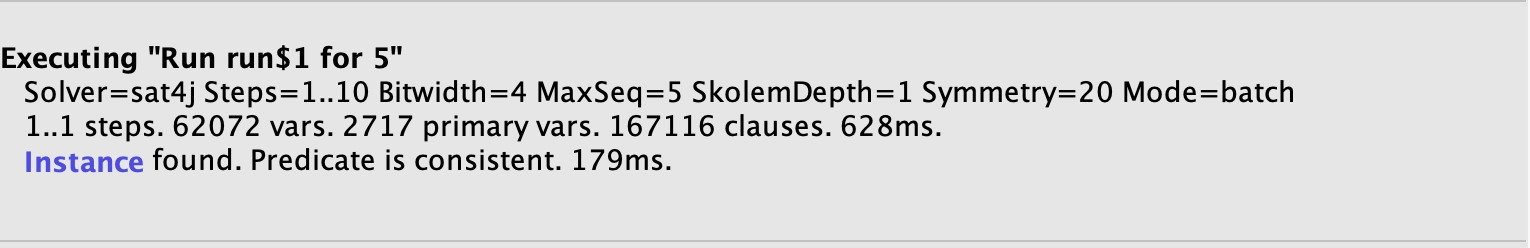
\includegraphics[scale=0.3]{Images/Alloy/alloyRun.jpeg}
   \\
  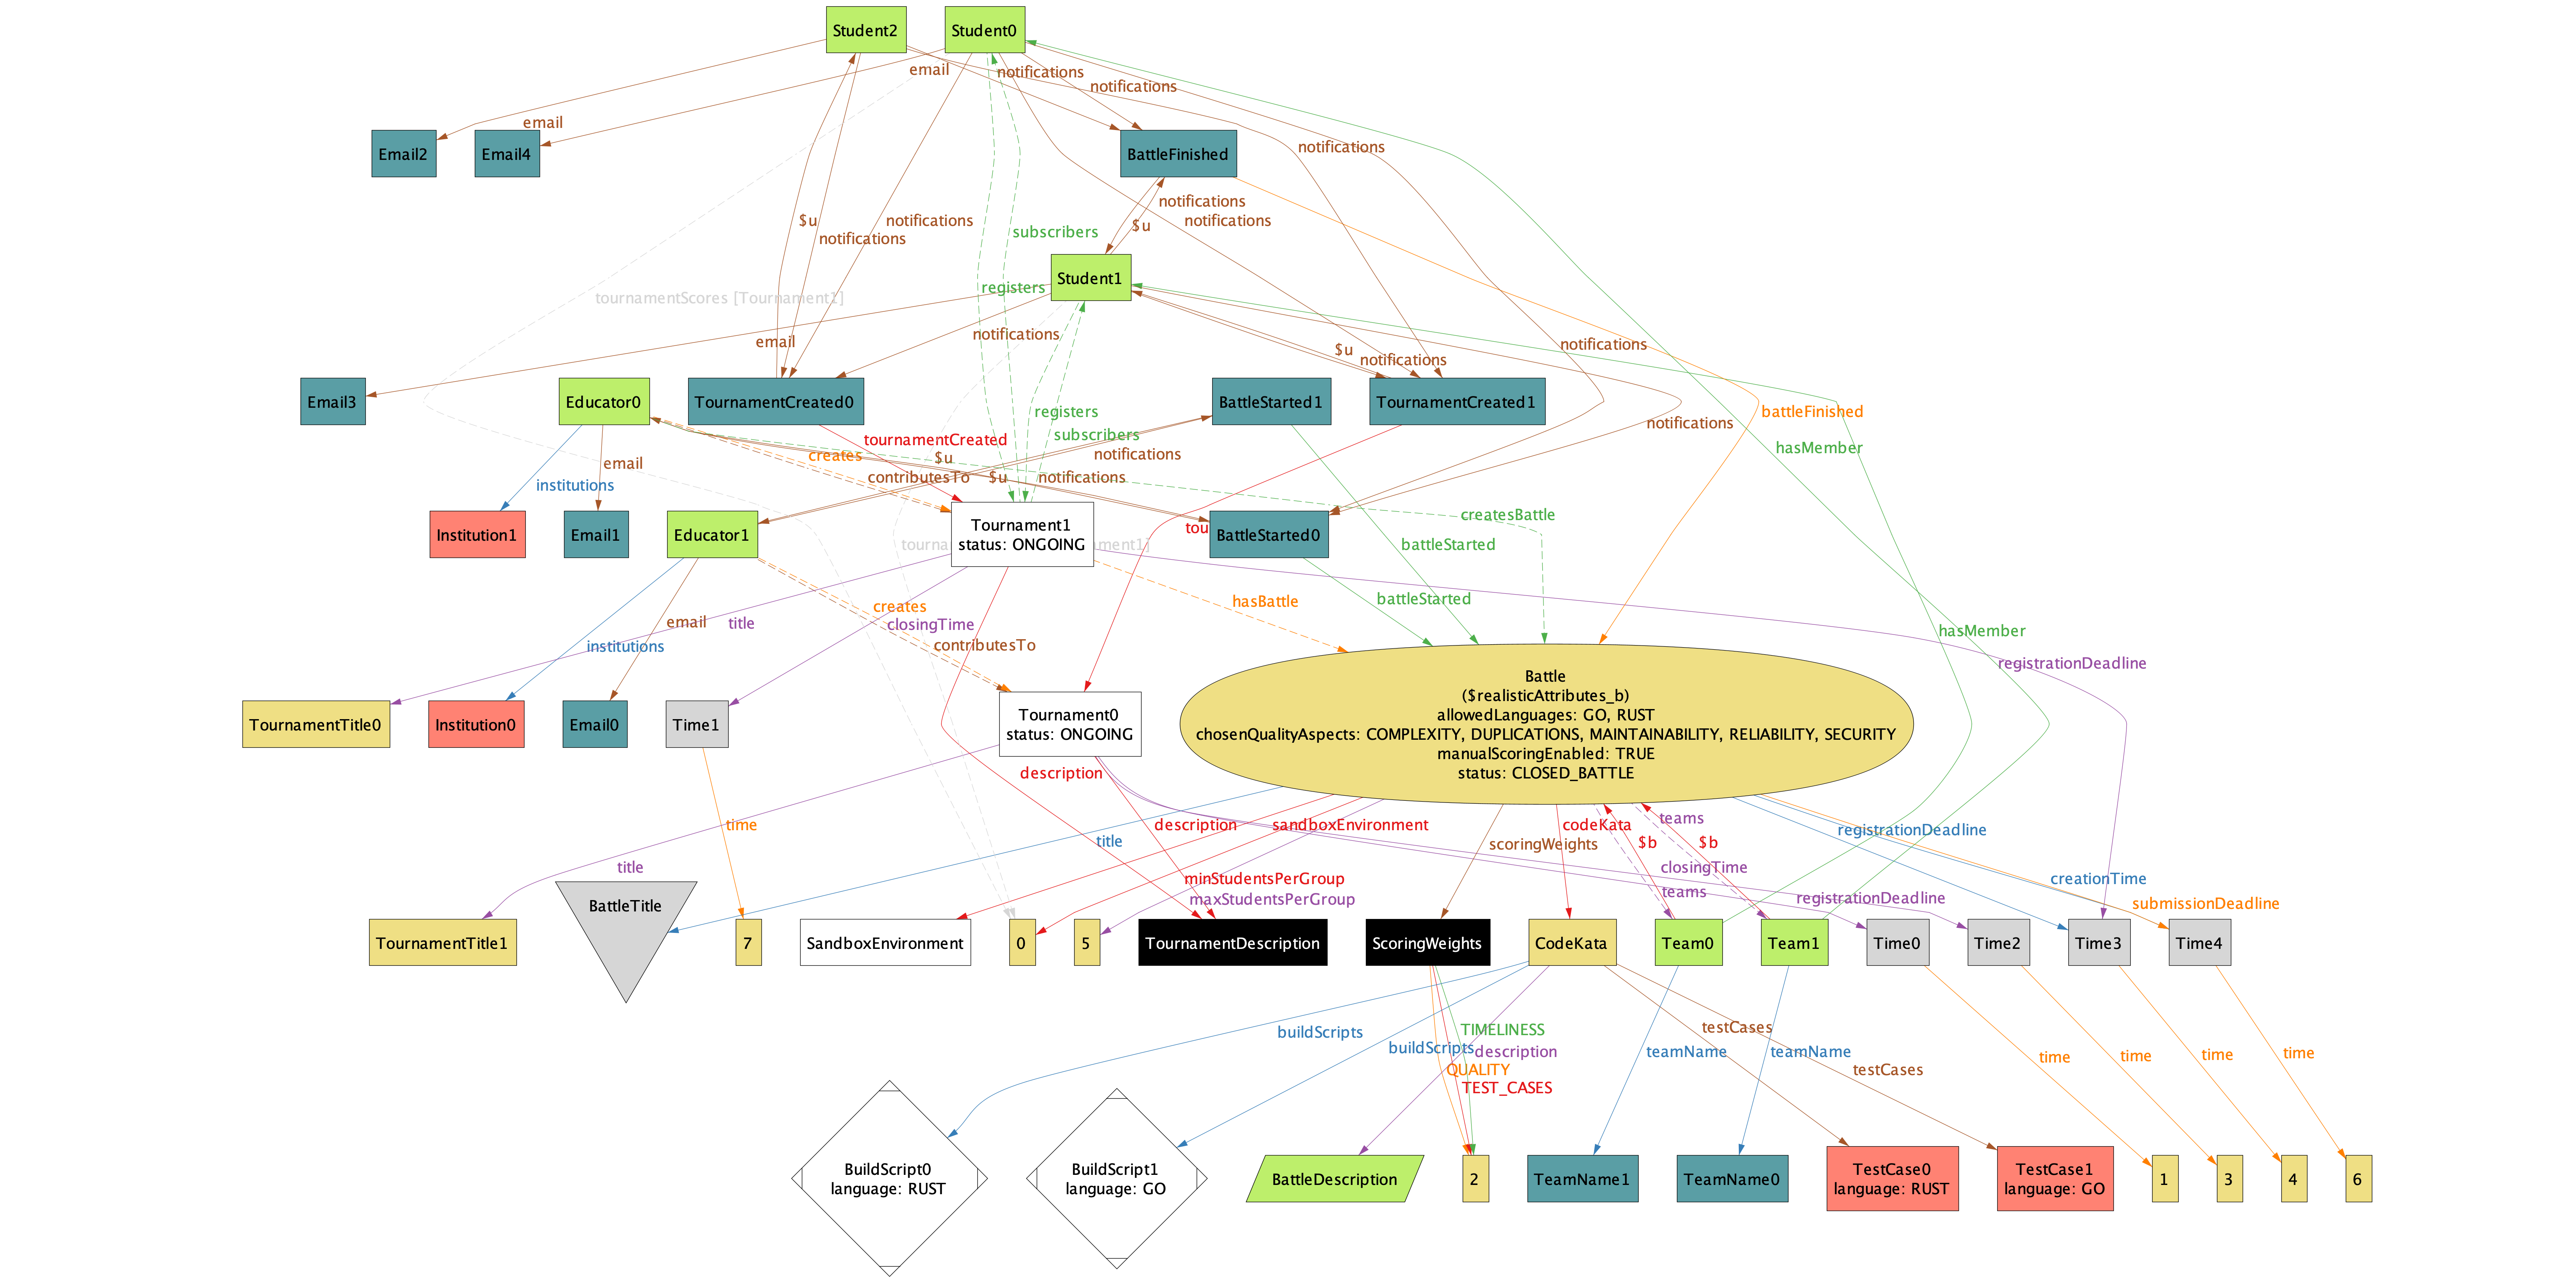
\includegraphics[scale=0.8]{Images/Alloy/World1_Alloy.png}

  \newpage
  \textbf{Dynamic Modelling}
  \\
     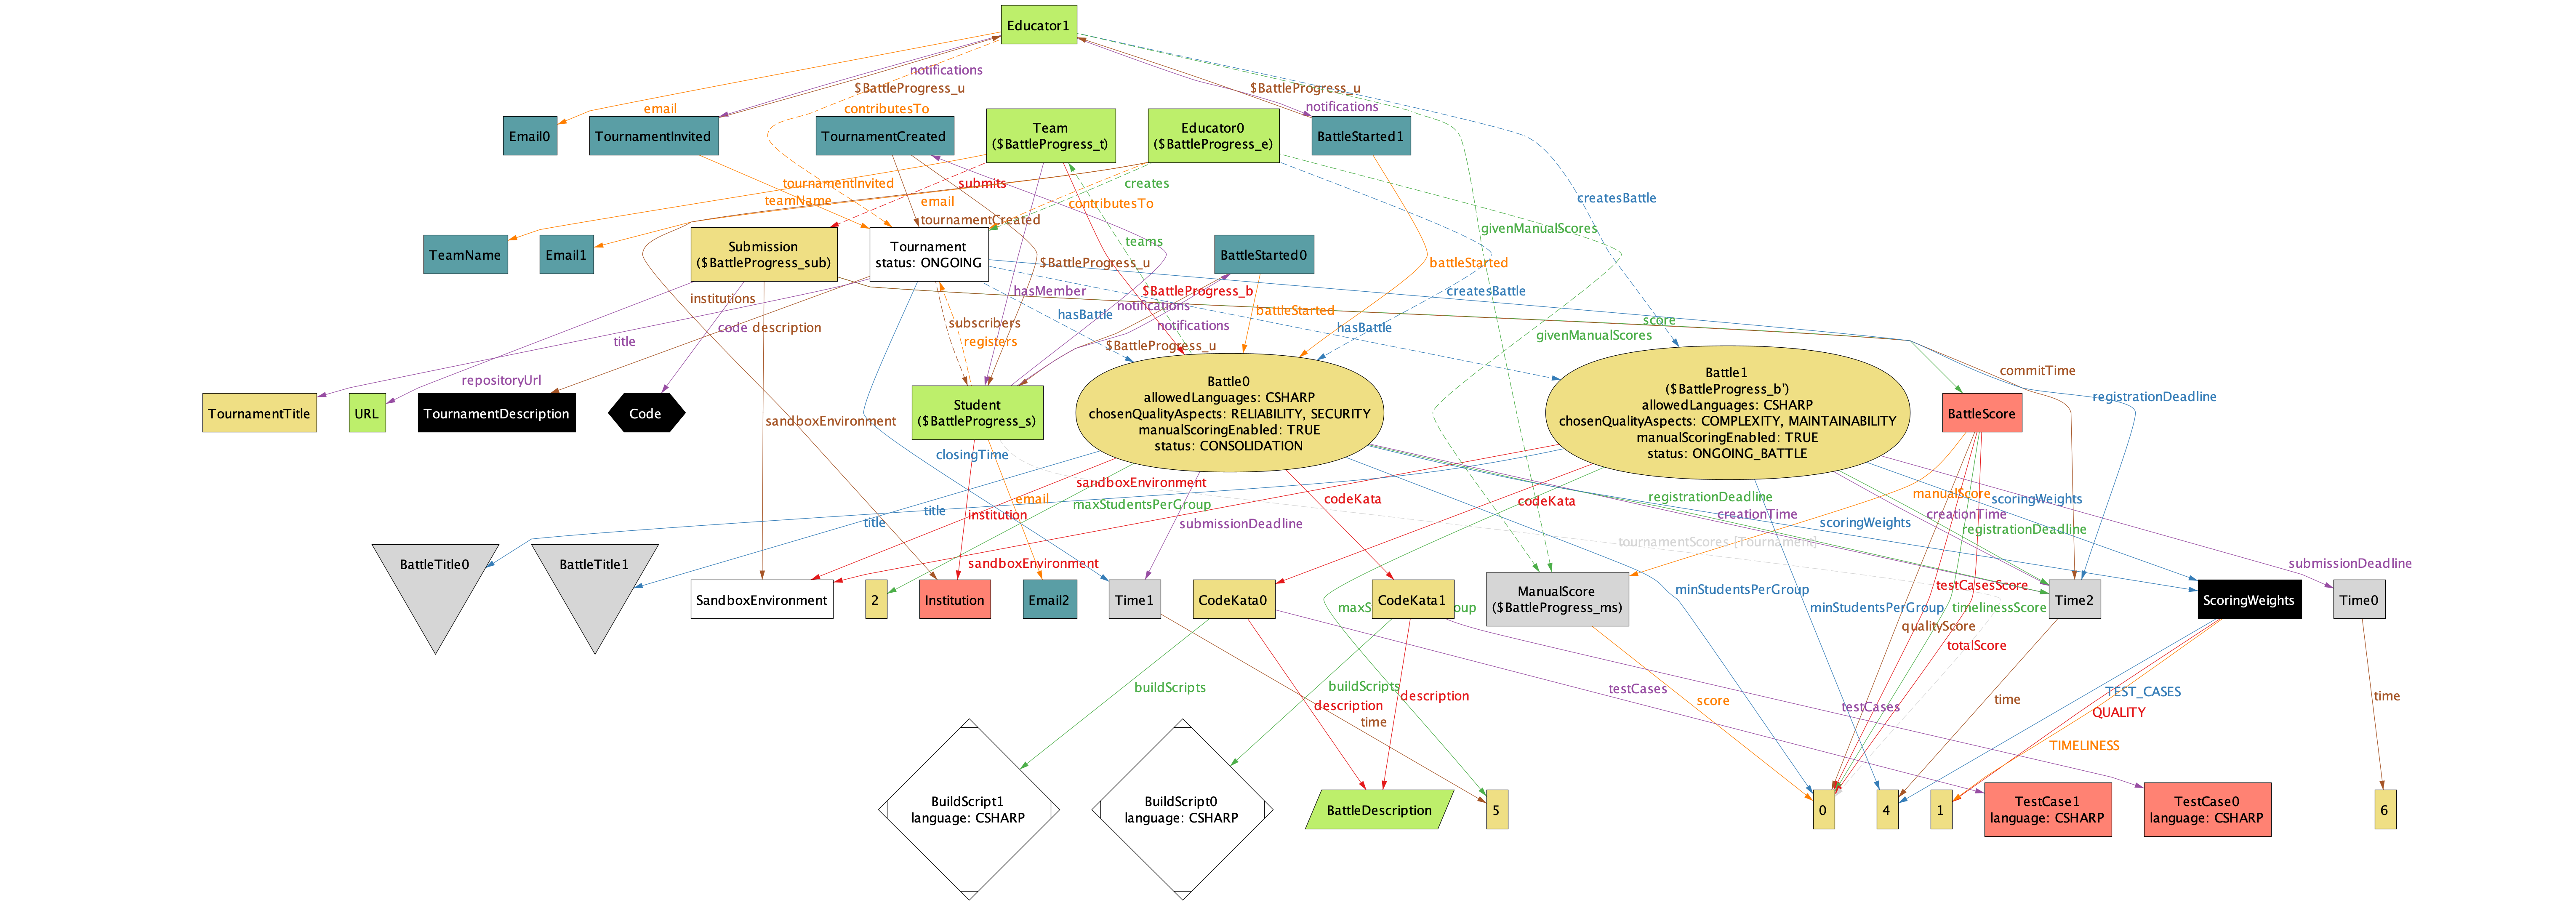
\includegraphics[scale=0.8]{Images/Alloy/Progress_1.png}
          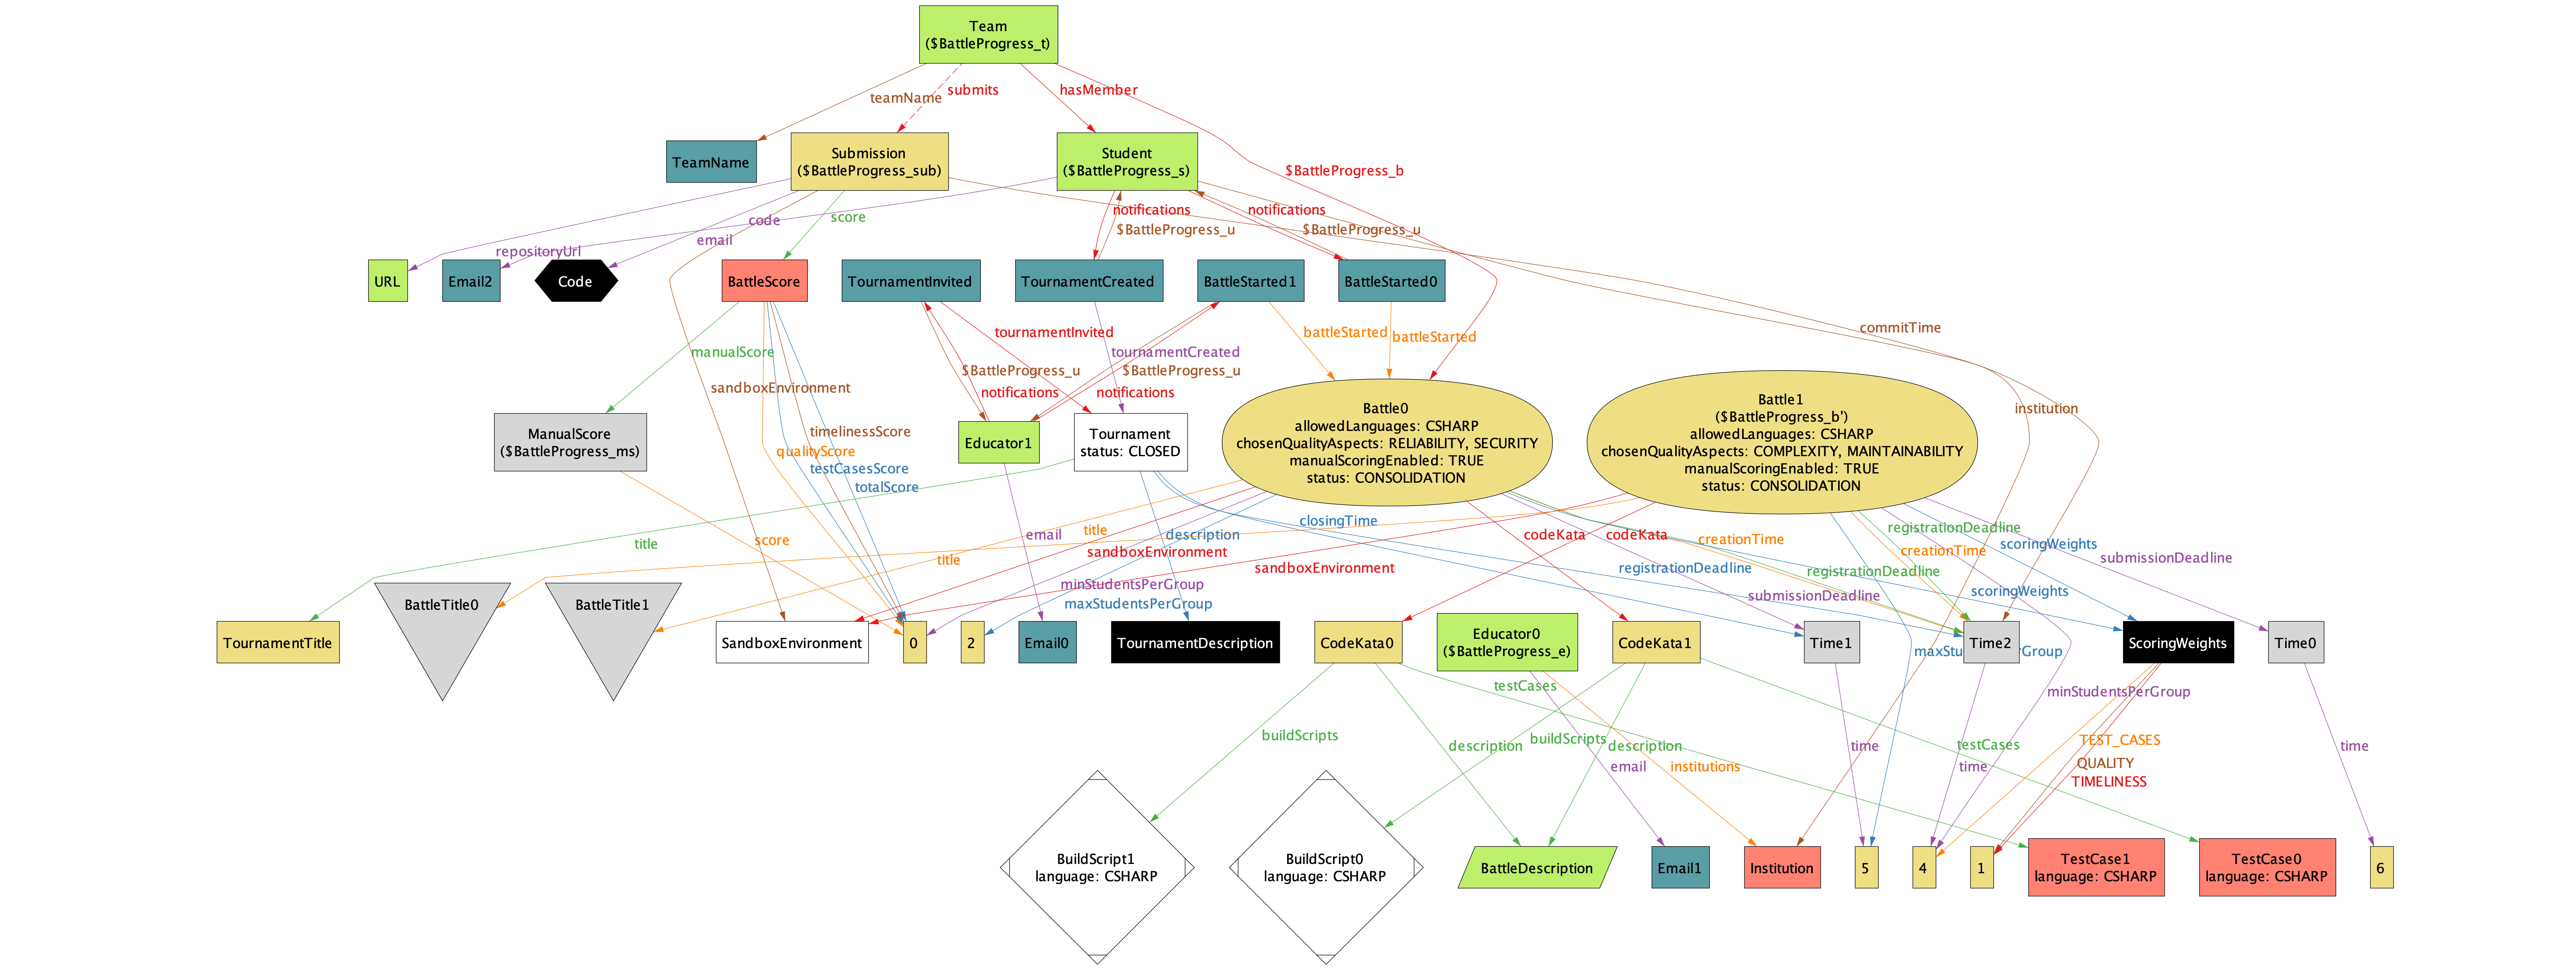
\includegraphics[scale=0.8]{Images/Alloy/Progress_2.png}
               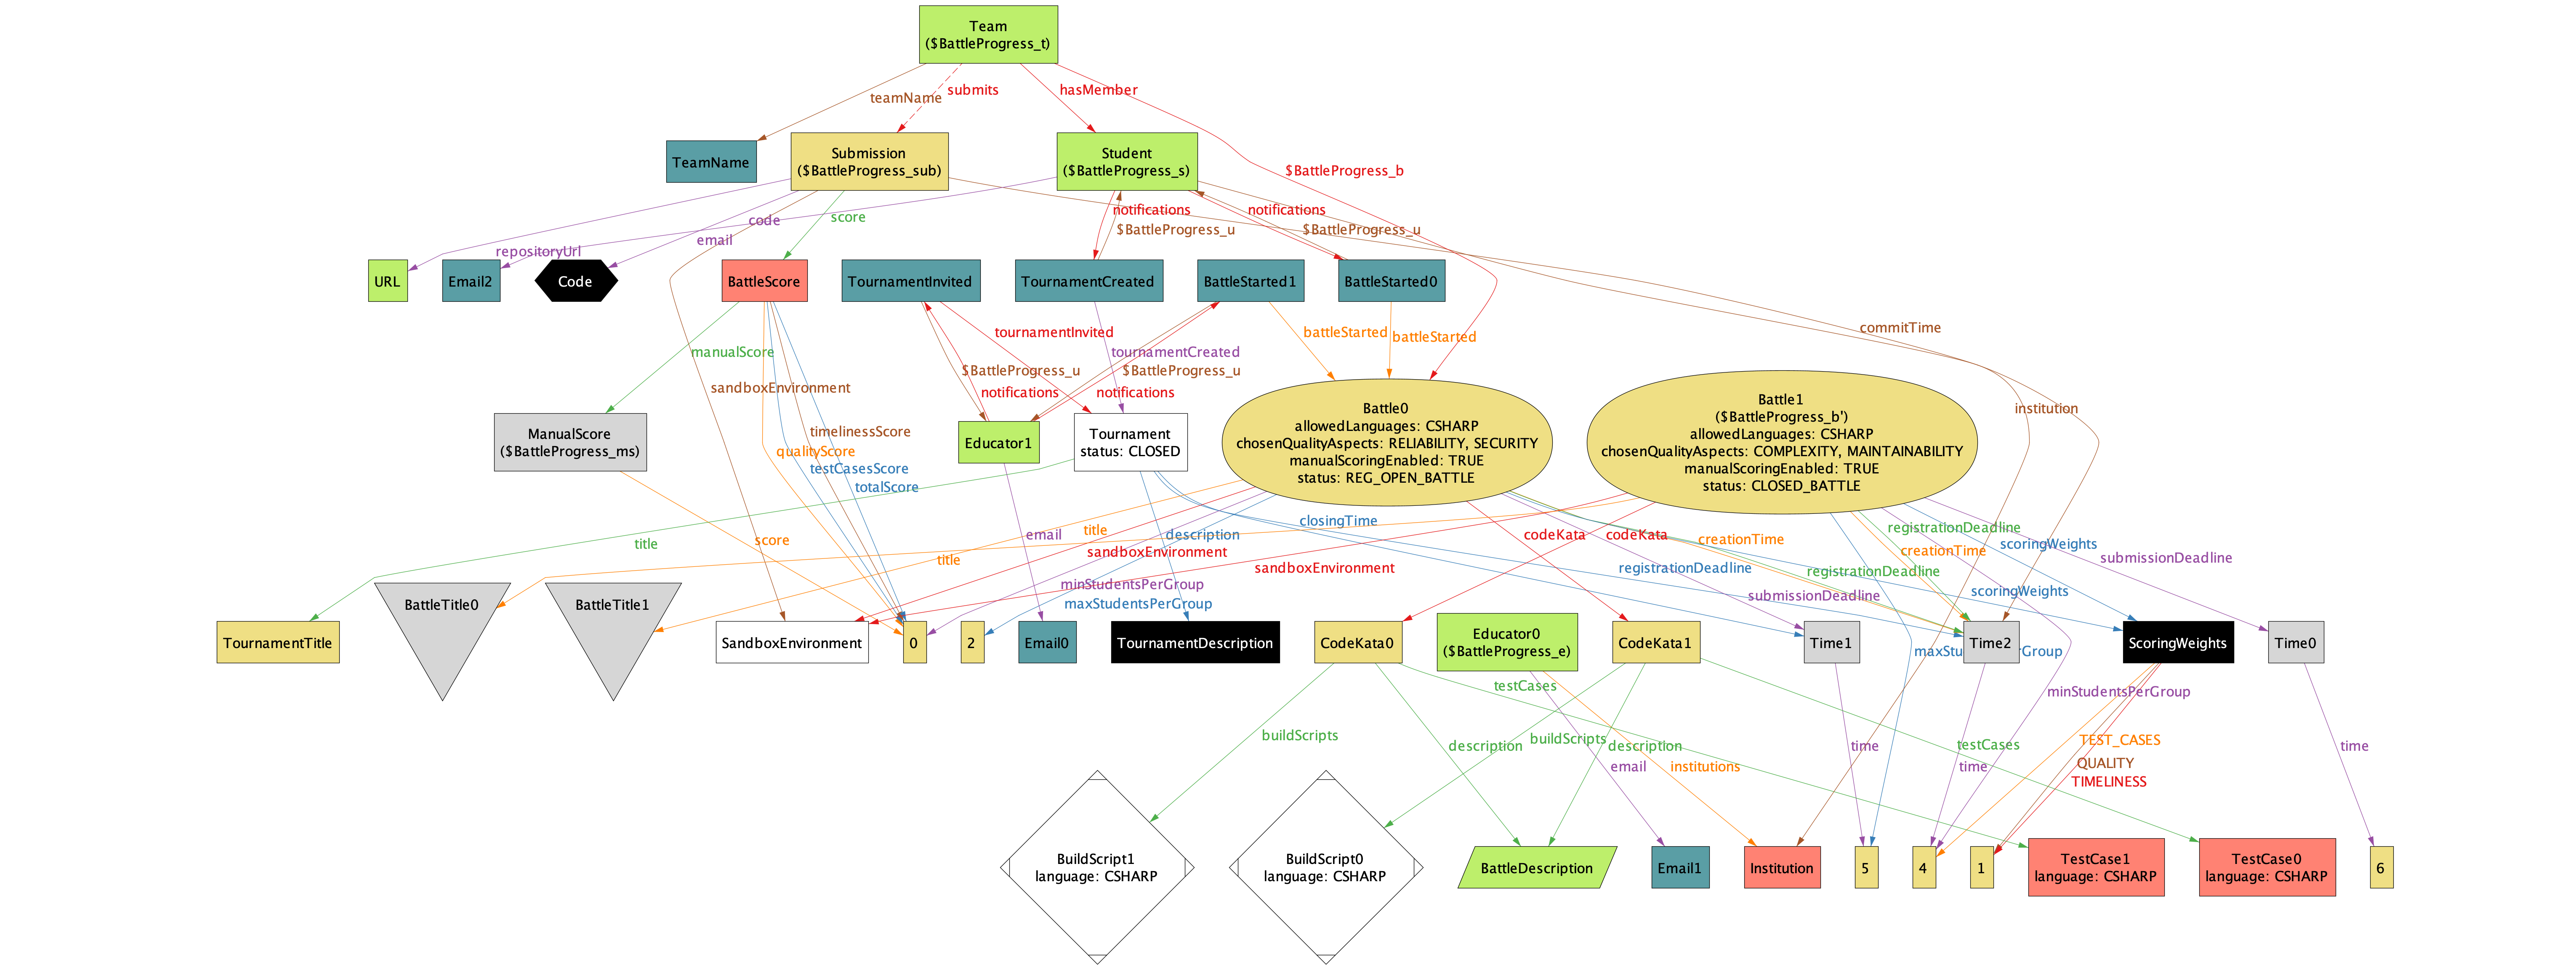
\includegraphics[scale=0.8]{Images/Alloy/Progress_3.png}